\documentclass[11pt]{article}
\usepackage{amsmath, amssymb, amsthm, geometry, graphicx, hyperref}
\usepackage{enumitem}
\usepackage{tikz}
\usetikzlibrary{arrows.meta, positioning}
\geometry{margin=1in}
\title{Zero-Knowledge Age Verification Protocol Using Pedersen Commitments}
\author{---}
\date{}

\begin{document}
\maketitle

\section{Overview}

This document describes a \textbf{basic} two-step protocol that enables a user to prove in zero knowledge that their age is greater than 18, based on a government-issued digital identity.  
The protocol uses \emph{Pedersen commitments} and \emph{range proofs} to achieve privacy-preserving age verification.

\vspace{1em}

The steps are:
\begin{enumerate}[label=\textbf{Step \arabic*:}]
  \item The user obtains a signed Pedersen commitment to their birthdate from a trusted authority.
  \item The user later proves to a verifier that the committed birthdate corresponds to an age $\ge 18$ without revealing the birthdate or any other information.
\end{enumerate}

\section{Preliminaries}

Let $G$ be a cyclic group of prime order $q$ with public generators $g,h \in G$ such that $\log_g h$ is unknown.  
The Pedersen commitment to a value $m \in \mathbb{Z}_q$ with randomness $r \in \mathbb{Z}_q$ is defined as:
\[
C = g^m h^r.
\]

This property is the key to our age-verification protocol.

\section{Step 1: Credential Issuance by the Authority}

\subsection{Goal}
Allow a user to obtain a cryptographically verifiable, privacy-preserving digital ID that commits to their birthdate.

\subsection{Protocol Description}

\begin{enumerate}[label=\arabic*)]
  \item The user computes a Pedersen commitment to their encoded birthdate:
  \[
  C = g^{b} h^{r},
  \]
  where:
  \begin{itemize}
    \item $b$ = user's birthdate encoded as an integer (e.g., days since epoch),
    \item $r$ = random blinding factor.
  \end{itemize}

  \item The user sends $C$ to the trusted authority, together with identifying information (in a secure and authenticated channel).

  \item The authority verifies the user’s real-world ID and signs the commitment:
  \[
  \sigma = \text{Sign}_{sk_A}(C, M),
  \]
  where $M$ is metadata (e.g., credential ID, expiry date, revocation handle).

  \item The authority returns the credential:
  \[
  \mathsf{Cred} = (C, \sigma, M).
  \]
\end{enumerate}

\subsection{Properties}
\begin{itemize}
  \item The authority attests that $C$ commits to the correct birthdate, but cannot later read $b$.
  \item The user can prove statements about $b$ without revealing it, using zero-knowledge proofs.
\end{itemize}

\section{Step 2: Zero-Knowledge Age Verification}

\subsection{Objective}
Given $(C, \sigma, M)$ and secret opening $(b,r)$, the user wants to convince a verifier that their age is greater than 18 without revealing $b$.

\subsection{Public Parameters}
\begin{itemize}
  \item Group $(G, q, g, h)$ as above.
  \item Authority’s public key $pk_A$ for verifying $\sigma$.
  \item Date encoding function $\text{encode\_date}(\cdot)$.
\end{itemize}

\subsection{Protocol}

\begin{enumerate}[label=\arabic*)]
  \item \textbf{Threshold computation:}  
  The verifier computes
  \[
  t = \text{encode\_date}(T - 18\ \text{years}),
  \]
  where $T$ is today’s date.

  \item \textbf{Construct commitment for the difference:}  
  The user computes
  \[
  D = g^{t} \cdot C^{-1} = g^{t - b} h^{-r}.
  \]
  Let $v = t - b$.  
  Then $D$ is a Pedersen commitment to $v$ with randomness $-r$.

  \item \textbf{Prove non-negativity:}  
  The user proves in zero knowledge that $v \in [0, 2^k)$ for some suitable bound $2^k$.  
  This ensures $t - b \ge 0$, i.e., $b \le t$.  

  The proof is a non-interactive \emph{range proof}:
  \[
  \pi \leftarrow \text{RangeProve}(D; v, -r, 2^k).
  \]

  \item \textbf{Send to verifier:}  
  The user sends $(C, \sigma, M, D, \pi)$.

  \item \textbf{Verifier checks:}
  \begin{enumerate}[label=\alph*)]
    \item Verify the authority signature $\sigma$ on $(C, M)$.
    \item Recompute $t$ and verify $D = g^{t} C^{-1}$.
    \item Verify the range proof $\pi$ using $\text{RangeVerify}(D, \pi, 2^k)$.
    \item Optionally check revocation/expiry in $M$.
  \end{enumerate}
\end{enumerate}

If all checks pass, the verifier is convinced that:
\begin{itemize}
  \item The credential was issued by a legitimate authority.
  \item The hidden birthdate $b$ satisfies $b \le t$ (i.e., age $\ge 18$).
  \item No additional personal information is revealed.
\end{itemize}

\subsection{Soundness and Zero-Knowledge}

\begin{itemize}
  \item \textbf{Soundness:}  
  The verifier is convinced that $b \le t$ only if the range proof is valid. Since the commitment is binding, the user cannot fake a younger age.
  \item \textbf{Zero-knowledge:}  
  Pedersen commitments and range proofs reveal nothing about $b$ or $r$. The verifier learns only that the age exceeds the threshold.
\end{itemize}

\subsection{Numeric Example (Illustrative Only)}

Let the group be modulo $p=23$ with generators $g=2$, $h=5$ (toy parameters).

\begin{align*}
T &= 100, \quad t = 82, \\
b &= 80, \quad r = 3, \\
C &= g^b h^r = 2^{80} \cdot 5^3 \pmod{23}, \\
D &= g^t C^{-1} = g^{2} h^{-3} = g^{t-b} h^{-r}.
\end{align*}

Here $v = t - b = 2$.  
A range proof shows that $v \in [0, 2^8)$, proving $b \le t$ (age $\ge 18$).

\subsection{Security and Implementation Notes}

\begin{itemize}
  \item Use secure elliptic-curve groups (e.g., Curve25519) and well-reviewed range-proof systems such as Bulletproofs.
  \item Ensure date encodings are bounded well below $q$ to avoid modular wraparound.
  \item Include domain separation and nonces in all Fiat–Shamir transcripts to prevent replay attacks.
  \item Support revocation through short credential lifetimes or cryptographic accumulators.
  \item For unlinkability across multiple verifiers, use blind or anonymous credential systems (e.g., BBS+, Idemix, CL signatures).
\end{itemize}

\subsection{Protocol Summary}

\begin{center}
\begin{tabular}{l|l}
\textbf{Step} & \textbf{Operation} \\
\hline
User & $C = g^{b} h^{r}$ \\
Authority & $\sigma = \text{Sign}_{sk_A}(C, M)$ \\
Verifier & Computes $t = \text{encode\_date}(T - 18\text{ years})$ \\
User & $D = g^{t} C^{-1}$ \\
User & $\pi = \text{RangeProve}(D; v=t-b)$ \\
User $\rightarrow$ Verifier & $(C, \sigma, M, D, \pi)$ \\
Verifier & Checks $\sigma$, $D=g^tC^{-1}$, and $\text{RangeVerify}(D, \pi)$
\end{tabular}
\end{center}

\section{Conclusion}

The presented protocol allows a user to prove that they are over 18 years old without disclosing their exact birthdate.  
It combines the perfect hiding and additive homomorphism of Pedersen commitments with zero-knowledge range proofs, producing a minimal and privacy-preserving age-verification mechanism suitable for integration with digital ID systems.

\section{Practical Cryptographic Recommendations}

This section summarizes the main cryptographic and operational recommendations for implementing the proposed age-verification zero-knowledge protocol securely and efficiently. The goal is to ensure both privacy and integrity during credential issuance (Step~1) and proof verification (Step~2).

\subsection{Group and Commitment Parameters}

\begin{itemize}
    \item \textbf{Group:} Use a prime-order elliptic-curve group, such as \texttt{secp256k1} or \texttt{Ed25519}, which offers efficient operations and well-audited libraries.
    \item \textbf{Generators:} Obtain independent generators $g, h$ deterministically via a hash-to-curve function to avoid trapdoors. Ensure that no party knows $\log_g h$.
    \item \textbf{Commitments:} Pedersen commitments $C = g^m h^r$ should be computed using cryptographically secure randomness for $r$. These commitments provide both \emph{hiding} and \emph{binding} properties.
\end{itemize}

\subsection{Authority Signature and Metadata}

\begin{itemize}
    \item \textbf{Digital Signature:} The issuing authority signs the hash of the commitment and credential metadata using a robust digital signature algorithm such as \texttt{Ed25519}, \texttt{ECDSA}, or \texttt{BLS}.
    \item \textbf{Metadata:} Include issuance time, expiry date, and a unique credential identifier within the signed data. This ensures verifiability and supports short-lived credentials.
    \item \textbf{Revocation:} Attach a revocation handle (e.g., the hash of a random revocation secret known to the authority) or maintain a revocation list/OCSP-like mechanism. Short-lived credentials can reduce the need for complex revocation checks.
\end{itemize}

\subsection{User Binding and Replay Prevention}

\begin{itemize}
    \item \textbf{Binding to User:} To prevent credential replay by unauthorized users, bind the credential to the user’s public key $PK_U$. The authority should sign the combined hash:
    \[
        \text{Sign}_{\text{Authority}}\big(H(C \| PK_U \| M)\big)
    \]
    where $M$ represents additional metadata. This approach slightly reduces unlinkability but increases theft-resistance.
    \item \textbf{Proof-of-Possession:} The authority must verify the user’s real-world identity and birth date during issuance. The user must demonstrate in zero-knowledge that the committed birth date used in the proof matches the one verified by the authority.
\end{itemize}

\subsection{Nonce and Expiry Management}

\begin{itemize}
    \item \textbf{Nonces:} Use nonces in challenge–response steps to prevent replay attacks in the zero-knowledge proof phase.
    \item \textbf{Expiry:} Credentials should include short validity periods to minimize the risk from compromised commitments or private keys.
\end{itemize}

\subsection{Implementation and Verification Tools}

\begin{itemize}
    \item \textbf{Formal Verification:} Use formal analysis tools such as \texttt{ProVerif}, \texttt{Tamarin}, or \texttt{F\textsuperscript{$\star$}} to verify key security properties including:
    \begin{itemize}
        \item \emph{Soundness:} Only users with valid commitments can pass verification.
        \item \emph{Zero-Knowledge:} No information about the user’s actual age is revealed beyond the statement “age $> 18$”.
        \item \emph{Unforgeability:} The credential cannot be fabricated or reused by others.
    \end{itemize}
\end{itemize}

\subsection{Summary of Design Properties}

The design ensures:
\begin{itemize}
    \item \textbf{Privacy:} No personal data (name, exact birthdate) is disclosed.
    \item \textbf{Integrity:} The verifier confirms the credential’s authenticity and issuance by a trusted authority.
    \item \textbf{Unlinkability:} Different proofs by the same user cannot be linked, provided $r$ and proof randomness are unique each time.
    \item \textbf{Non-Forgeability:} Without the private key or correct commitment randomness, generating a valid proof is infeasible.
\end{itemize}

\section{To the Next Level: Advanced Design Enhancements}

Beyond the foundational protocol and basic security recommendations, several refinements can elevate the age-verification system from a conceptual prototype to a production-grade privacy infrastructure. These address practical deployment, interoperability, and resistance to subtle cryptographic pitfalls.

\subsection{Elliptic Curve and Parameter Hardening}

\begin{itemize}
    \item \textbf{Curve Choice:} Adopt a modern, secure elliptic curve such as \texttt{Curve25519} or \texttt{secp256k1}, depending on compatibility requirements. These curves are well-studied and have efficient implementations in multiple languages.
    \item \textbf{Generator Derivation:} Derive generators $g, h$ deterministically using a \emph{hash-to-curve} function to eliminate trust assumptions. Ensure that no entity can compute $\log_g h$.
    \item \textbf{Encoding and Domain Parameters:} Choose encoding and field parameters so committed values remain small and avoid modular wrap-around when used in range or comparison proofs.
\end{itemize}

\subsection{Advanced Zero-Knowledge Components}

\begin{itemize}
    \item \textbf{Range Proofs:} Integrate a well-audited range proof system such as \texttt{Bulletproofs} or \texttt{LegoSNARKs} to ensure committed ages are non-negative and within realistic bounds.
    \item \textbf{Comparison Proofs:} Optimize the “age $>18$” comparison using modular decomposition (binary representation) or constraint systems compatible with the chosen ZK backend.
\end{itemize}

\subsection{Revocation and Credential Lifecycle}

\begin{itemize}
    \item \textbf{Revocation Strategy:} Define a robust revocation mechanism. Options include:
    \begin{enumerate}
        \item Time-bounded credentials with short expiry.
        \item Revocation lists or status servers (OCSP-like).
        \item Cryptographic accumulators for scalable privacy-preserving revocation.
    \end{enumerate}
    \item \textbf{Expiry Policy:} Encourage periodic credential renewal to mitigate key compromise or metadata leakage.
\end{itemize}

\subsection{Privacy and Linkability Policy}

\begin{itemize}
    \item \textbf{Anonymous vs. Linkable Credentials:} Decide early whether the system should allow multiple proofs from the same credential to be unlinkable. 
    \item \textbf{Techniques:} Employ credential blinding or anonymous credentials (e.g., based on BBS+ or CL signatures) if unlinkability is a requirement. For regulated environments, controlled linkability may be acceptable.
\end{itemize}

\subsection{Hash Domain Separation and Context Binding}

\begin{itemize}
    \item \textbf{Domain Separation:} Introduce unique prefixes or tags in every hash used in Fiat–Shamir transformations or commitment derivations to avoid cross-protocol replay or collision with other systems.
    \item \textbf{Context Binding:} Include protocol version, service domain, and verifier identity within the hash transcript to ensure proofs are valid only in their intended context.
\end{itemize}

\subsection{Integration and Security Verification}

\begin{itemize}
    \item \textbf{Formal Verification:} Model the full protocol in \texttt{ProVerif}, \texttt{Tamarin}, or \texttt{F\textsuperscript{\⋆}} to analyze confidentiality, soundness, and unlinkability.
    \item \textbf{Implementation Review:} Conduct independent audits focusing on randomness generation, nonce uniqueness, and memory safety in proof libraries.
    \item \textbf{Interoperability:} Use standardized serialization formats (CBOR, JSON-LD, or DID-compatible structures) to integrate with digital identity frameworks such as W3C Verifiable Credentials.
\end{itemize}

\subsection{Outcome}

Incorporating these enhancements yields a protocol that is:
\begin{itemize}
    \item Cryptographically hardened against subtle parameter misuse.
    \item Extensible to richer ZK credential ecosystems.
    \item Compatible with revocation, policy, and interoperability layers.
    \item Securely bound to its application context and resistant to replay or linkage attacks.
\end{itemize}

\section{Diagram}

\begin{figure}[h!]
\centering
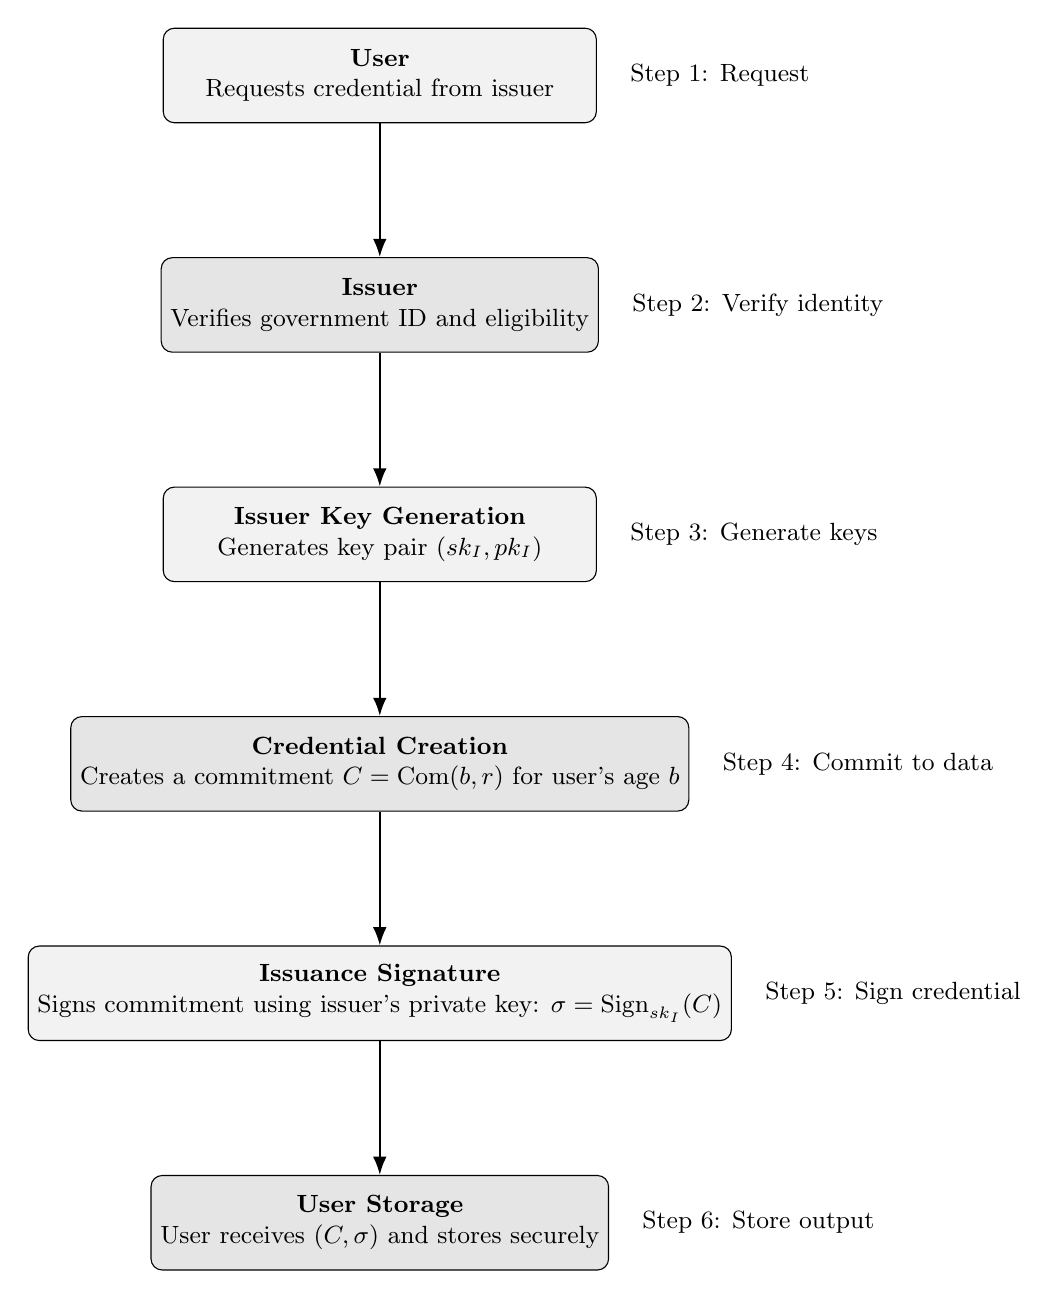
\begin{tikzpicture}[
  node distance=1.7cm,
  box/.style={
    rectangle,
    draw,
    rounded corners,
    align=center,
    minimum width=5.5cm,
    minimum height=1.2cm,
    fill=gray!10
  },
  arrow/.style={-Latex, thick},
  every node/.append style={font=\small}
]

% Nodes (stacked top-down)
\node[box, fill=gray!10] (user) {\textbf{User} \\ Requests credential from issuer};
\node[box, fill=gray!20, below=of user] (issuer) {\textbf{Issuer} \\ Verifies government ID and eligibility};
\node[box, fill=gray!10, below=of issuer] (keygen) {\textbf{Issuer Key Generation} \\ Generates key pair $(sk_I, pk_I)$};
\node[box, fill=gray!20, below=of keygen] (cred) {\textbf{Credential Creation} \\ Creates a commitment $C = \text{Com}(b, r)$ for user's age $b$};
\node[box, fill=gray!10, below=of cred] (sign) {\textbf{Issuance Signature} \\ Signs commitment using issuer’s private key: $\sigma = \text{Sign}_{sk_I}(C)$};
\node[box, fill=gray!20, below=of sign] (store) {\textbf{User Storage} \\ User receives $(C, \sigma)$ and stores securely};

% Arrows
\draw[arrow] (user) -- (issuer);
\draw[arrow] (issuer) -- (keygen);
\draw[arrow] (keygen) -- (cred);
\draw[arrow] (cred) -- (sign);
\draw[arrow] (sign) -- (store);

% Optional labels for flow
\node[right=0.3cm of user.east, align=left] {Step 1: Request};
\node[right=0.3cm of issuer.east, align=left] {Step 2: Verify identity};
\node[right=0.3cm of keygen.east, align=left] {Step 3: Generate keys};
\node[right=0.3cm of cred.east, align=left] {Step 4: Commit to data};
\node[right=0.3cm of sign.east, align=left] {Step 5: Sign credential};
\node[right=0.3cm of store.east, align=left] {Step 6: Store output};

\end{tikzpicture}
\caption{Step 2 – Getting Digital ID using Pedersen Commitments}
\label{fig:age-verification}
\end{figure}


\begin{figure}[h!]
\centering
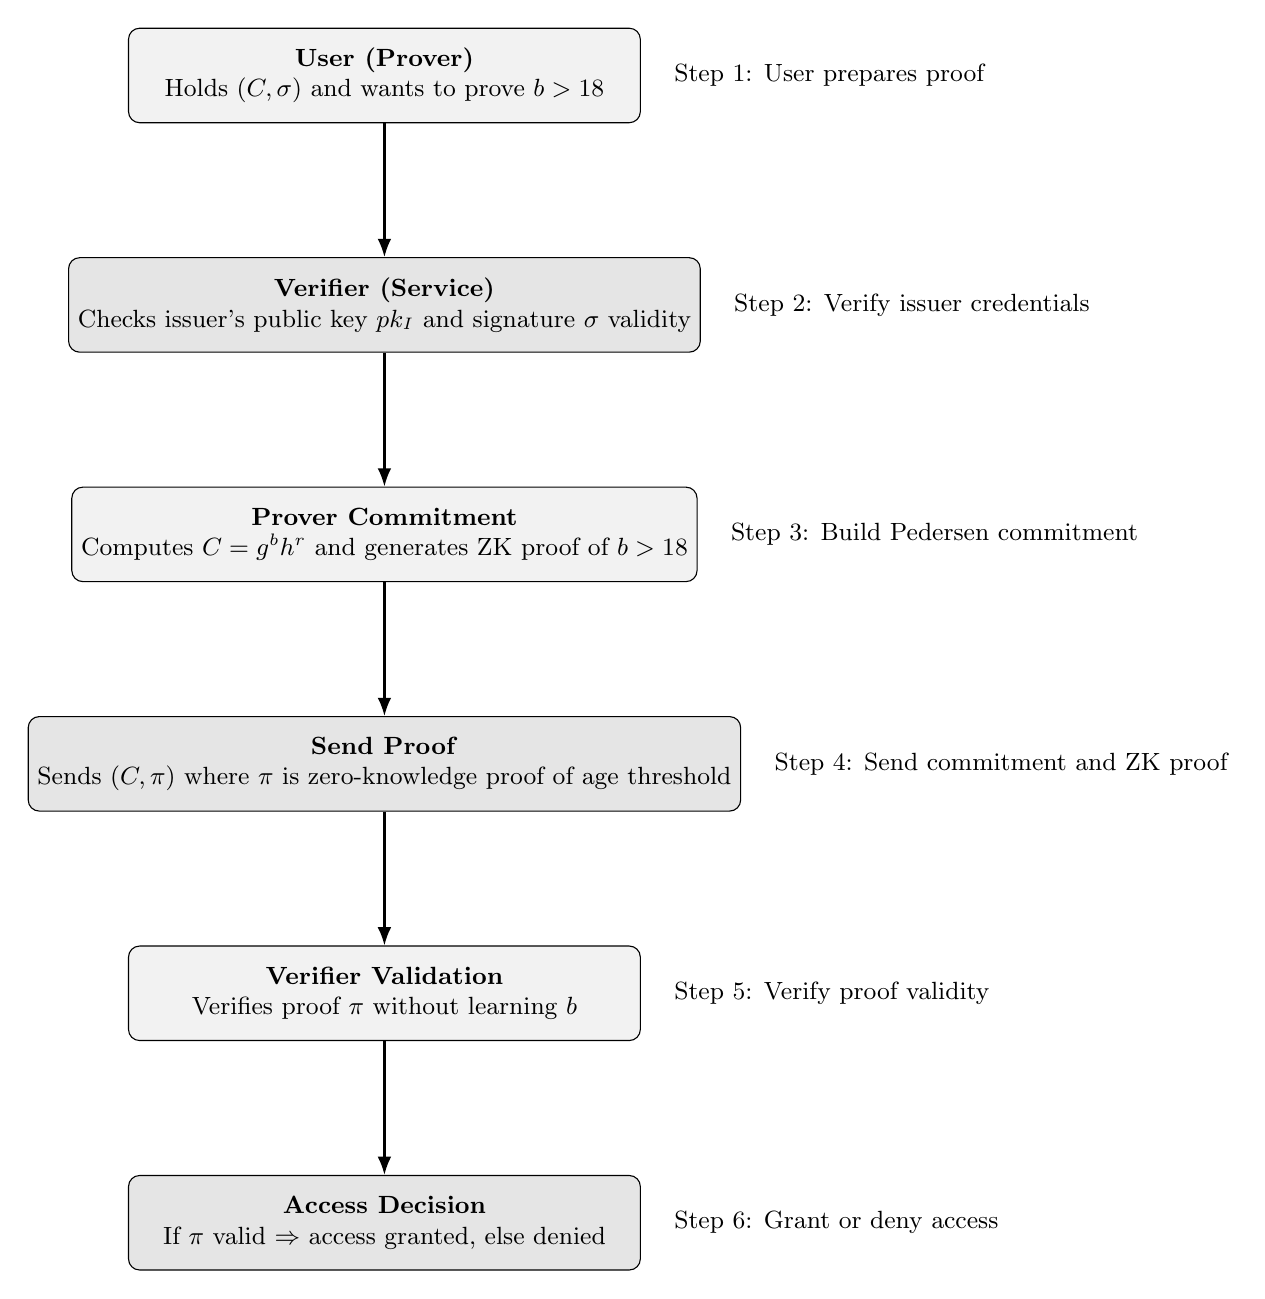
\begin{tikzpicture}[
  node distance=1.7cm,
  box/.style={
    rectangle,
    draw,
    rounded corners,
    align=center,
    minimum width=6.5cm,
    minimum height=1.2cm,
    fill=gray!10
  },
  arrow/.style={-Latex, thick},
  every node/.append style={font=\small}
]

% Nodes (stacked top-down)
\node[box, fill=gray!10] (user) {\textbf{User (Prover)} \\ Holds $(C, \sigma)$ and wants to prove $b > 18$};
\node[box, fill=gray!20, below=of user] (verifySig) {\textbf{Verifier (Service)} \\ Checks issuer’s public key $pk_I$ and signature $\sigma$ validity};
\node[box, fill=gray!10, below=of verifySig] (commit) {\textbf{Prover Commitment} \\ Computes $C = g^b h^r$ and generates ZK proof of $b > 18$};
\node[box, fill=gray!20, below=of commit] (proofSend) {\textbf{Send Proof} \\ Sends $(C, \pi)$ where $\pi$ is zero-knowledge proof of age threshold};
\node[box, fill=gray!10, below=of proofSend] (verifyProof) {\textbf{Verifier Validation} \\ Verifies proof $\pi$ without learning $b$};
\node[box, fill=gray!20, below=of verifyProof] (result) {\textbf{Access Decision} \\ If $\pi$ valid $\Rightarrow$ access granted, else denied};

% Arrows
\draw[arrow] (user) -- (verifySig);
\draw[arrow] (verifySig) -- (commit);
\draw[arrow] (commit) -- (proofSend);
\draw[arrow] (proofSend) -- (verifyProof);
\draw[arrow] (verifyProof) -- (result);

% Optional right-hand labels
\node[right=0.3cm of user.east, align=left] {Step 1: User prepares proof};
\node[right=0.3cm of verifySig.east, align=left] {Step 2: Verify issuer credentials};
\node[right=0.3cm of commit.east, align=left] {Step 3: Build Pedersen commitment};
\node[right=0.3cm of proofSend.east, align=left] {Step 4: Send commitment and ZK proof};
\node[right=0.3cm of verifyProof.east, align=left] {Step 5: Verify proof validity};
\node[right=0.3cm of result.east, align=left] {Step 6: Grant or deny access};

\end{tikzpicture}
\caption{Step 2 – Zero-Knowledge Age Verification Protocol using Pedersen Commitments}
\label{fig:age-verification}
\end{figure}




\end{document}
